\section{The Circular Polarized Alfven Wave Test}

In this sample we run the circular polarized Alfven wave test as descriped
on the Athena test page\footnote{
\url{http://www.astro.princeton.edu/~jstone/Athena/tests/cp-alfven-wave/cp-alfven.html}}
by Jim Stone.
In this setup, the density is $\rho=1$ and the pressure is $p=0.1$,
and the ratio of specific heats is $\gamma=5/3$.
In the {\sc Pencil Code}, this is achieved with $\ln\rho=s=0$
by setting $\csz$ such that $\csz^2=\gamma p/\rho=5\times0.1/3\approx0.16666667$,
i.e., $\csz\approx0.40824829$.

We consider a two-dimensional domain, $0\leq x<2$ and $0\leq y<1$.
Furthermore, velocity and magnetic field perturbations are equal to
each other, such that the components in the $xy$ plane are
\EQ
\uu_\perp=\BB_\perp=0.1\sin\kk\cdot\xx,
\EN
where $\kk=(\pi,2\pi,0)$.
The $z$ components are given by
\EQ
u_z=B_z=0.1\cos\kk\cdot\xx.
\EN
Since $\kk=(\pi,2\pi,0)$, we have $|\kk|=\sqrt{5}\pi$ and
\begin{equation}
\AAA=\pmatrix{0\cr A_{y0}\sin(k_xx+k_yy)\cr A_{z0}\cos(k_xx+k_yy)}
\end{equation}
where $A_{z0}=0.1|\kk|^{-1}\approx0.014235251$.
$A_{y0}\approx0.031830989$.

\begin{figure}[t!]\begin{center}
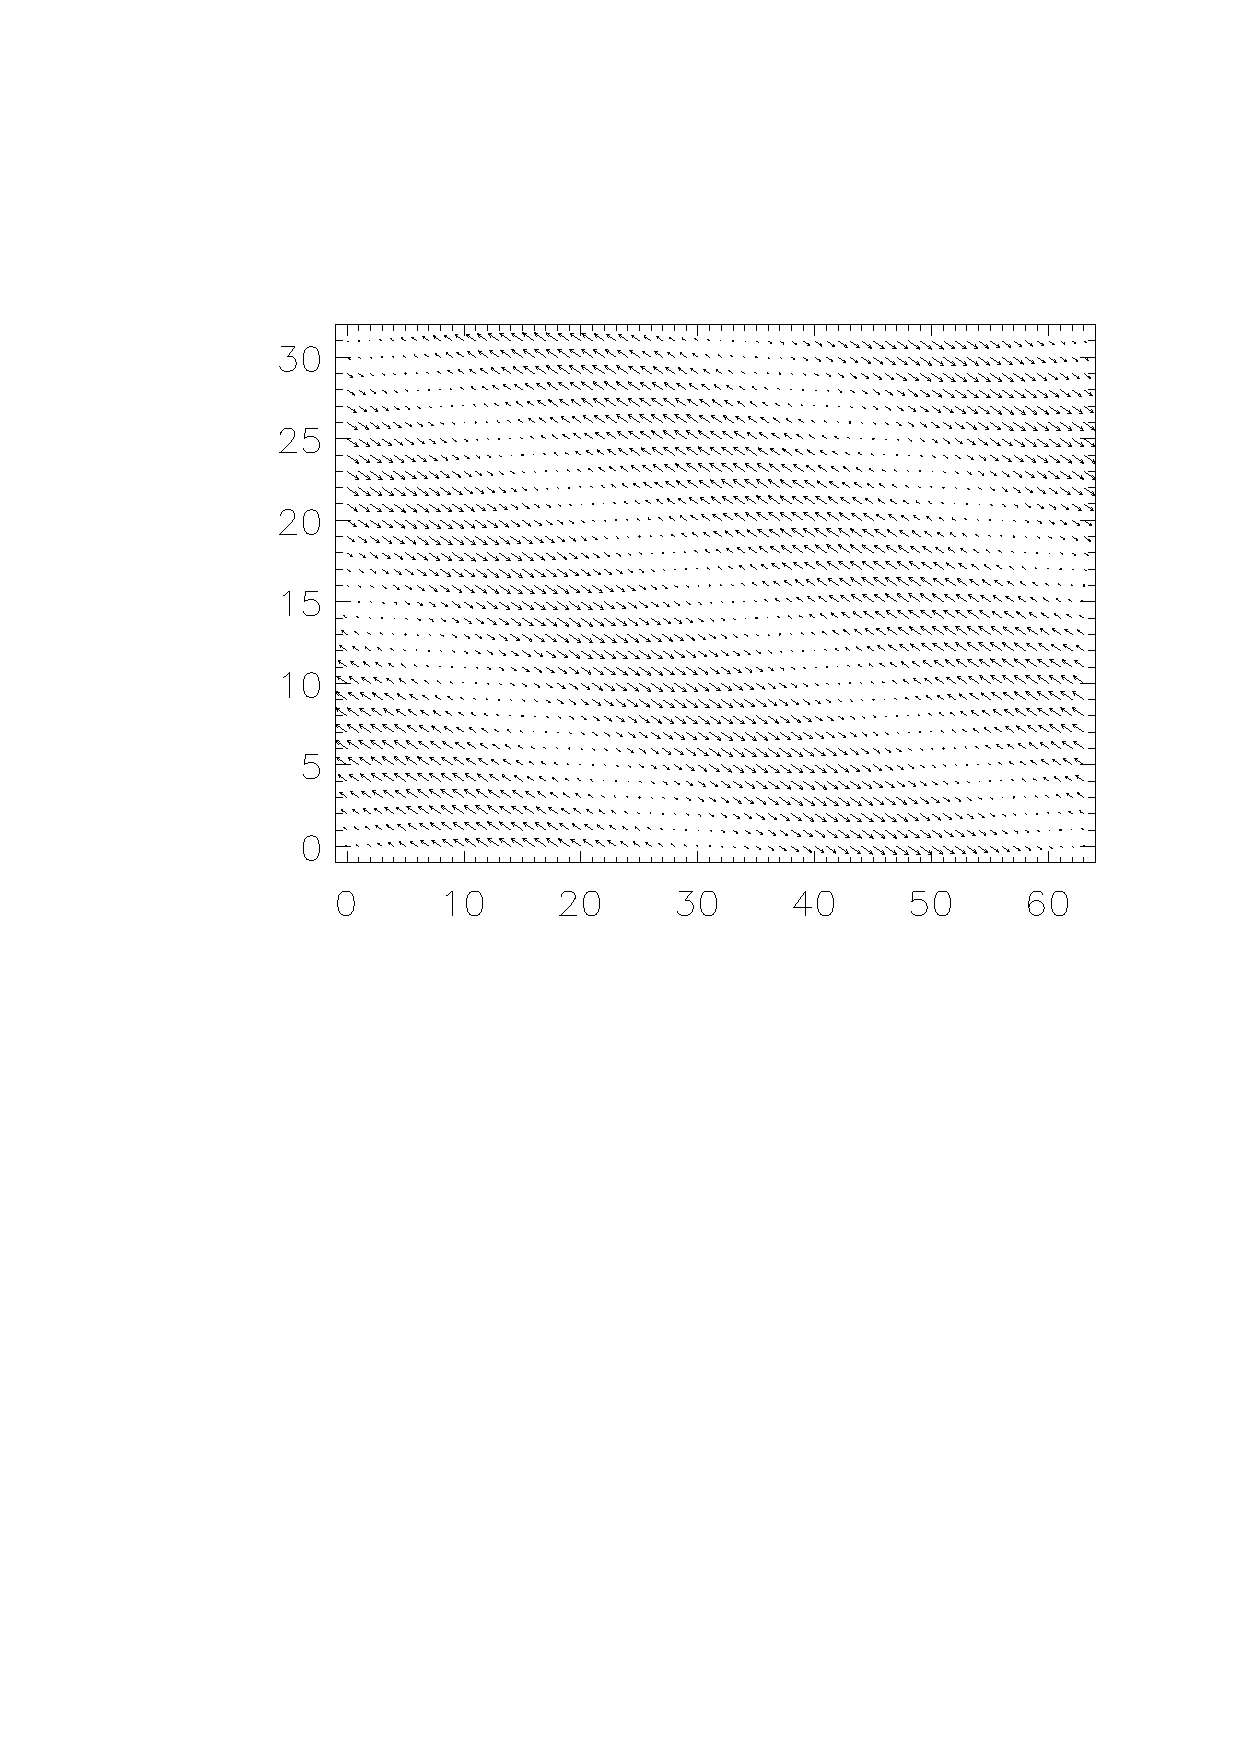
\includegraphics[width=\columnwidth]{pvar}
\end{center}\caption[]{
Perturbation
}\label{pvar}\end{figure}

%\begin{table}[htb]\caption{
%}\vspace{12pt}\centerline{\begin{tabular}{lccccccc}
%\hline
%\label{Ttimescale}\end{tabular}}\end{table}

\begin{verbatim}
\end{verbatim}

%\begin{itemize}
%\item
%\end{itemize}
